\documentclass[a4paper]{book}
\usepackage{makeidx}
\usepackage{graphicx}
\usepackage{multicol}
\usepackage{float}
\usepackage{listings}
\usepackage{color}
\usepackage{ifthen}
\usepackage[table]{xcolor}
\usepackage{textcomp}
\usepackage{alltt}
\usepackage{ifpdf}
\ifpdf
\usepackage[pdftex,
            pagebackref=true,
            colorlinks=true,
            linkcolor=blue,
            unicode
           ]{hyperref}
\else
\usepackage[ps2pdf,
            pagebackref=true,
            colorlinks=true,
            linkcolor=blue,
            unicode
           ]{hyperref}
\usepackage{pspicture}
\fi
\usepackage[utf8]{inputenc}
\usepackage{mathptmx}
\usepackage[scaled=.90]{helvet}
\usepackage{courier}
\usepackage{sectsty}
\usepackage[titles]{tocloft}
\usepackage{doxygen}
\lstset{language=C++,inputencoding=utf8,basicstyle=\footnotesize,breaklines=true,breakatwhitespace=true,tabsize=8,numbers=left }
\makeindex
\setcounter{tocdepth}{3}
\renewcommand{\footrulewidth}{0.4pt}
\renewcommand{\familydefault}{\sfdefault}
\begin{document}
\hypersetup{pageanchor=false}
\begin{titlepage}
\vspace*{7cm}
\begin{center}
{\Large BayPHP \\[1ex]\large 0.1 }\\
\vspace*{1cm}
{\large Generated by Doxygen 1.7.4}\\
\vspace*{0.5cm}
{\small Sat Jan 28 2012 11:36:01}\\
\end{center}
\end{titlepage}
\clearemptydoublepage
\pagenumbering{roman}
\tableofcontents
\clearemptydoublepage
\pagenumbering{arabic}
\hypersetup{pageanchor=true}
\chapter{Class Index}
\section{Class Hierarchy}
This inheritance list is sorted roughly, but not completely, alphabetically:\begin{DoxyCompactList}
\item \contentsline{section}{Account}{\pageref{classAccount}}{}
\item \contentsline{section}{Exception}{\pageref{classException}}{}
\begin{DoxyCompactList}
\item \contentsline{section}{AccountException}{\pageref{classAccountException}}{}
\item \contentsline{section}{FileException}{\pageref{classFileException}}{}
\end{DoxyCompactList}
\item \contentsline{section}{File}{\pageref{classFile}}{}
\item \contentsline{section}{Request}{\pageref{classRequest}}{}
\item \contentsline{section}{Uploader}{\pageref{classUploader}}{}
\end{DoxyCompactList}

\chapter{Class Index}
\section{Class List}
Here are the classes, structs, unions and interfaces with brief descriptions:\begin{DoxyCompactList}
\item\contentsline{section}{\hyperlink{classAccount}{Account} (Retrieves data about bayfiles accounts by sending requests to \href{http://api.bayfiles.com/v1/account/}{\tt http://api.bayfiles.com/v1/account/} )}{\pageref{classAccount}}{}
\item\contentsline{section}{\hyperlink{classAccountException}{AccountException} (\hyperlink{classAccountException}{AccountException} occurs when requesting /account fails )}{\pageref{classAccountException}}{}
\item\contentsline{section}{\hyperlink{classException}{Exception} (Base exception class )}{\pageref{classException}}{}
\item\contentsline{section}{\hyperlink{classFile}{File} (Retrieves data about bayfiles files by sending requests to \href{http://api.bayfiles.com/v1/account/}{\tt http://api.bayfiles.com/v1/account/} )}{\pageref{classFile}}{}
\item\contentsline{section}{\hyperlink{classFileException}{FileException} (\hyperlink{classFileException}{FileException} occurs when requesting /file fails )}{\pageref{classFileException}}{}
\item\contentsline{section}{\hyperlink{classRequest}{Request} (Sends http requests to the Bayfiles API )}{\pageref{classRequest}}{}
\item\contentsline{section}{\hyperlink{classUploader}{Uploader} (Class for uploading files )}{\pageref{classUploader}}{}
\end{DoxyCompactList}

\chapter{Class Documentation}
\hypertarget{classAccount}{
\section{Account Class Reference}
\label{classAccount}\index{Account@{Account}}
}


Retrieves data about bayfiles accounts by sending requests to \href{http://api.bayfiles.com/v1/account/.}{\tt http://api.bayfiles.com/v1/account/.}  


\subsection*{Public Member Functions}
\begin{DoxyCompactItemize}
\item 
\hyperlink{classAccount_ada0eeeed16967d6e548488030b5bdaef}{\_\-\_\-construct} (\$username, \$password)
\begin{DoxyCompactList}\small\item\em \hyperlink{classAccount}{Account} construct. \end{DoxyCompactList}\item 
\hyperlink{classAccount_aadd43a144ad6802e0fa8967e437fd8bb}{getUsername} ()
\begin{DoxyCompactList}\small\item\em user name getter \end{DoxyCompactList}\item 
\hyperlink{classAccount_ad94891116350680172a3c2529d7f0570}{getPassword} ()
\begin{DoxyCompactList}\small\item\em password getter \end{DoxyCompactList}\item 
\hyperlink{classAccount_a3b37b3393454a1352929b4010ac8e9c3}{getSession} ()
\begin{DoxyCompactList}\small\item\em sends a request to /account/info if the session string is not cached yet and returns it \end{DoxyCompactList}\item 
\hyperlink{classAccount_ace3c3419f3683e4a0a0dba26bd91a194}{getEmail} ()
\begin{DoxyCompactList}\small\item\em sends a request to /account/info if the email is not cached yet and returns it \end{DoxyCompactList}\item 
\hypertarget{classAccount_a07d537af3b7de4caffa58c1a67763966}{
\hyperlink{classAccount_a07d537af3b7de4caffa58c1a67763966}{getFilesCount} ()}
\label{classAccount_a07d537af3b7de4caffa58c1a67763966}

\begin{DoxyCompactList}\small\item\em sends a request to /account/info if the files count is not cached yet and returns it \end{DoxyCompactList}\item 
\hyperlink{classAccount_acead8f2ef19395aeae6a8ab94e21e50b}{getStorage} ()
\begin{DoxyCompactList}\small\item\em sends a request to /account/info if the session string is not cached yet and returns it \end{DoxyCompactList}\item 
\hypertarget{classAccount_af1c983ce957b5e181633c2aff278d15f}{
\hyperlink{classAccount_af1c983ce957b5e181633c2aff278d15f}{isPremium} ()}
\label{classAccount_af1c983ce957b5e181633c2aff278d15f}

\begin{DoxyCompactList}\small\item\em sends a request to /account/info if the premiumness is not cached yet and returns it \end{DoxyCompactList}\item 
\hypertarget{classAccount_a5f7f8ff34b4befbf757455e8011d1832}{
\hyperlink{classAccount_a5f7f8ff34b4befbf757455e8011d1832}{getExpires} ()}
\label{classAccount_a5f7f8ff34b4befbf757455e8011d1832}

\begin{DoxyCompactList}\small\item\em sends a request to /account/info if the session string is not cached yet and returns it \end{DoxyCompactList}\item 
\hypertarget{classAccount_a84a49c7e2888e8cff244e25e1901d5d3}{
\hyperlink{classAccount_a84a49c7e2888e8cff244e25e1901d5d3}{getCodes} ()}
\label{classAccount_a84a49c7e2888e8cff244e25e1901d5d3}

\begin{DoxyCompactList}\small\item\em sends a request to /account/info if the number of codes is not cached yet and returns it \end{DoxyCompactList}\item 
\hyperlink{classAccount_aa0dc98ce30abcd3d1a73c1a3e123a544}{getFiles} ()
\begin{DoxyCompactList}\small\item\em sends a request to /account/files if this request has not been done yet. \end{DoxyCompactList}\item 
\hypertarget{classAccount_a6a7ff1d886d9eb0894a71481912a59e5}{
\hyperlink{classAccount_a6a7ff1d886d9eb0894a71481912a59e5}{editPassword} (\$value)}
\label{classAccount_a6a7ff1d886d9eb0894a71481912a59e5}

\begin{DoxyCompactList}\small\item\em sends a request to /account/edit/password/(password) to edit the password \end{DoxyCompactList}\item 
\hypertarget{classAccount_ad20b13631f56caa944b0791b4a0f648c}{
\hyperlink{classAccount_ad20b13631f56caa944b0791b4a0f648c}{editEmail} (\$value)}
\label{classAccount_ad20b13631f56caa944b0791b4a0f648c}

\begin{DoxyCompactList}\small\item\em sends a request to /account/edit/email/(email) to edit the email \end{DoxyCompactList}\item 
\hypertarget{classAccount_a1dee4bb90b333fe6628d7898f8b50972}{
\hyperlink{classAccount_a1dee4bb90b333fe6628d7898f8b50972}{login} ()}
\label{classAccount_a1dee4bb90b333fe6628d7898f8b50972}

\begin{DoxyCompactList}\small\item\em sends a request to /account/login/(username)/(password) \end{DoxyCompactList}\item 
\hypertarget{classAccount_a14df93ec30cd4bd0d7f3df839ce6e4d5}{
\hyperlink{classAccount_a14df93ec30cd4bd0d7f3df839ce6e4d5}{logout} ()}
\label{classAccount_a14df93ec30cd4bd0d7f3df839ce6e4d5}

\begin{DoxyCompactList}\small\item\em sends a request to /account/logout \end{DoxyCompactList}\end{DoxyCompactItemize}


\subsection{Detailed Description}
Retrieves data about bayfiles accounts by sending requests to \href{http://api.bayfiles.com/v1/account/.}{\tt http://api.bayfiles.com/v1/account/.} 

Definition at line 10 of file account.php.



\subsection{Constructor \& Destructor Documentation}
\hypertarget{classAccount_ada0eeeed16967d6e548488030b5bdaef}{
\index{Account@{Account}!\_\-\_\-construct@{\_\-\_\-construct}}
\index{\_\-\_\-construct@{\_\-\_\-construct}!Account@{Account}}
\subsubsection[{\_\-\_\-construct}]{\setlength{\rightskip}{0pt plus 5cm}Account::\_\-\_\-construct (
\begin{DoxyParamCaption}
\item[{\$}]{username, }
\item[{\$}]{password}
\end{DoxyParamCaption}
)}}
\label{classAccount_ada0eeeed16967d6e548488030b5bdaef}


\hyperlink{classAccount}{Account} construct. 


\begin{DoxyParams}{Parameters}
{\em username} & username \\
\hline
{\em password} & password \\
\hline
\end{DoxyParams}


Definition at line 31 of file account.php.



\subsection{Member Function Documentation}
\hypertarget{classAccount_ace3c3419f3683e4a0a0dba26bd91a194}{
\index{Account@{Account}!getEmail@{getEmail}}
\index{getEmail@{getEmail}!Account@{Account}}
\subsubsection[{getEmail}]{\setlength{\rightskip}{0pt plus 5cm}Account::getEmail (
\begin{DoxyParamCaption}
{}
\end{DoxyParamCaption}
)}}
\label{classAccount_ace3c3419f3683e4a0a0dba26bd91a194}


sends a request to /account/info if the email is not cached yet and returns it 

\begin{DoxyReturn}{Returns}
email 
\end{DoxyReturn}


Definition at line 86 of file account.php.

\hypertarget{classAccount_aa0dc98ce30abcd3d1a73c1a3e123a544}{
\index{Account@{Account}!getFiles@{getFiles}}
\index{getFiles@{getFiles}!Account@{Account}}
\subsubsection[{getFiles}]{\setlength{\rightskip}{0pt plus 5cm}Account::getFiles (
\begin{DoxyParamCaption}
{}
\end{DoxyParamCaption}
)}}
\label{classAccount_aa0dc98ce30abcd3d1a73c1a3e123a544}


sends a request to /account/files if this request has not been done yet. 

\begin{DoxyReturn}{Returns}
array of bay$\backslash$File(s) 
\end{DoxyReturn}


Definition at line 140 of file account.php.

\hypertarget{classAccount_ad94891116350680172a3c2529d7f0570}{
\index{Account@{Account}!getPassword@{getPassword}}
\index{getPassword@{getPassword}!Account@{Account}}
\subsubsection[{getPassword}]{\setlength{\rightskip}{0pt plus 5cm}Account::getPassword (
\begin{DoxyParamCaption}
{}
\end{DoxyParamCaption}
)}}
\label{classAccount_ad94891116350680172a3c2529d7f0570}


password getter 

\begin{DoxyReturn}{Returns}
password 
\end{DoxyReturn}


Definition at line 64 of file account.php.

\hypertarget{classAccount_a3b37b3393454a1352929b4010ac8e9c3}{
\index{Account@{Account}!getSession@{getSession}}
\index{getSession@{getSession}!Account@{Account}}
\subsubsection[{getSession}]{\setlength{\rightskip}{0pt plus 5cm}Account::getSession (
\begin{DoxyParamCaption}
{}
\end{DoxyParamCaption}
)}}
\label{classAccount_a3b37b3393454a1352929b4010ac8e9c3}


sends a request to /account/info if the session string is not cached yet and returns it 

\begin{DoxyReturn}{Returns}
session string 
\end{DoxyReturn}


Definition at line 76 of file account.php.

\hypertarget{classAccount_acead8f2ef19395aeae6a8ab94e21e50b}{
\index{Account@{Account}!getStorage@{getStorage}}
\index{getStorage@{getStorage}!Account@{Account}}
\subsubsection[{getStorage}]{\setlength{\rightskip}{0pt plus 5cm}Account::getStorage (
\begin{DoxyParamCaption}
{}
\end{DoxyParamCaption}
)}}
\label{classAccount_acead8f2ef19395aeae6a8ab94e21e50b}


sends a request to /account/info if the session string is not cached yet and returns it 

\begin{DoxyReturn}{Returns}
storage 
\end{DoxyReturn}


Definition at line 104 of file account.php.

\hypertarget{classAccount_aadd43a144ad6802e0fa8967e437fd8bb}{
\index{Account@{Account}!getUsername@{getUsername}}
\index{getUsername@{getUsername}!Account@{Account}}
\subsubsection[{getUsername}]{\setlength{\rightskip}{0pt plus 5cm}Account::getUsername (
\begin{DoxyParamCaption}
{}
\end{DoxyParamCaption}
)}}
\label{classAccount_aadd43a144ad6802e0fa8967e437fd8bb}


user name getter 

\begin{DoxyReturn}{Returns}
user name 
\end{DoxyReturn}


Definition at line 54 of file account.php.



The documentation for this class was generated from the following file:\begin{DoxyCompactItemize}
\item 
bayphp/account.php\end{DoxyCompactItemize}

\hypertarget{classAccountException}{
\section{AccountException Class Reference}
\label{classAccountException}\index{AccountException@{AccountException}}
}


\hyperlink{classAccountException}{AccountException} occurs when requesting /account fails.  


Inheritance diagram for AccountException:\begin{figure}[H]
\begin{center}
\leavevmode
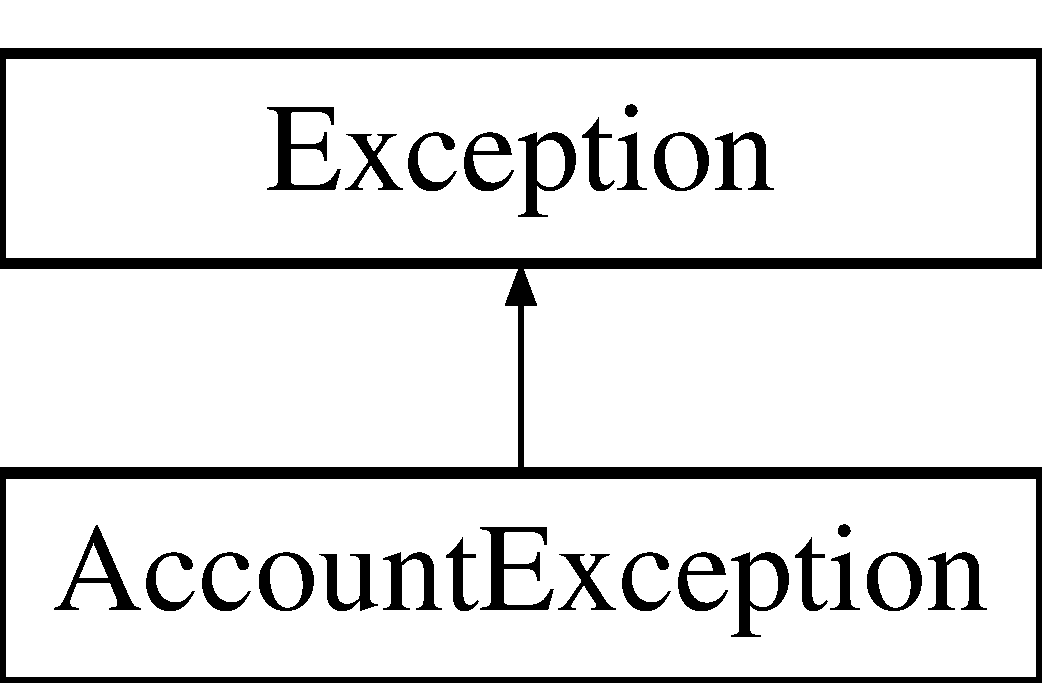
\includegraphics[height=2.000000cm]{classAccountException}
\end{center}
\end{figure}


\subsection{Detailed Description}
\hyperlink{classAccountException}{AccountException} occurs when requesting /account fails. 

Definition at line 28 of file exceptions.php.



The documentation for this class was generated from the following file:\begin{DoxyCompactItemize}
\item 
bayphp/exceptions.php\end{DoxyCompactItemize}

\hypertarget{classException}{
\section{Exception Class Reference}
\label{classException}\index{Exception@{Exception}}
}


base exception class  


Inheritance diagram for Exception:\begin{figure}[H]
\begin{center}
\leavevmode
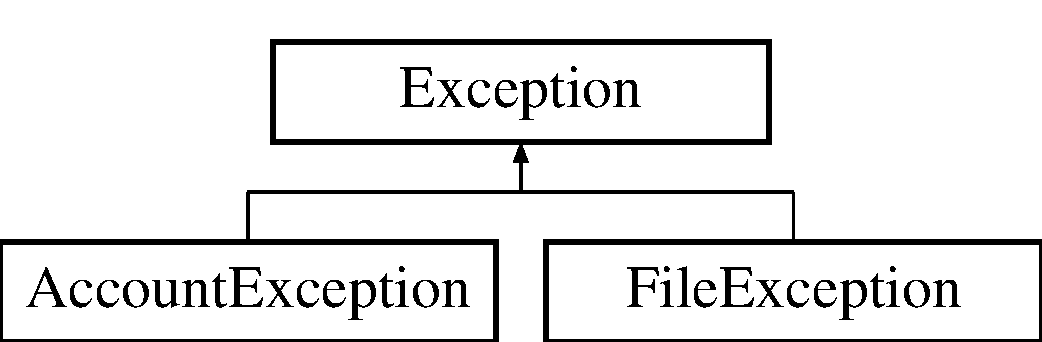
\includegraphics[height=2.000000cm]{classException}
\end{center}
\end{figure}
\subsection*{Public Member Functions}
\begin{DoxyCompactItemize}
\item 
\hypertarget{classException_a84cb308cbcf072fe19e9e2b8ec83918e}{
\hyperlink{classException_a84cb308cbcf072fe19e9e2b8ec83918e}{\_\-\_\-toString} ()}
\label{classException_a84cb308cbcf072fe19e9e2b8ec83918e}

\begin{DoxyCompactList}\small\item\em standard serializer method \end{DoxyCompactList}\end{DoxyCompactItemize}


\subsection{Detailed Description}
base exception class 

These exceptions contain error message given by Bayfiles most of the time. They may be thrown by a wrong usage of BayPHP, for example if you try to delete a file without its delete token, the request is not even attempted. 

Definition at line 14 of file exceptions.php.



The documentation for this class was generated from the following file:\begin{DoxyCompactItemize}
\item 
bayphp/exceptions.php\end{DoxyCompactItemize}

\hypertarget{classFile}{
\section{File Class Reference}
\label{classFile}\index{File@{File}}
}


Retrieves data about bayfiles files by sending requests to \href{http://api.bayfiles.com/v1/account/.}{\tt http://api.bayfiles.com/v1/account/.}  


\subsection*{Public Member Functions}
\begin{DoxyCompactItemize}
\item 
\hyperlink{classFile_ad6ff8555973b48a3448ac72b57d8eb0c}{\_\-\_\-construct} (\$fileId, \$infoToken, \$deleteToken=null, \$size=null, \$sha1=null, \$name=null, \$owner=null)
\begin{DoxyCompactList}\small\item\em \hyperlink{classFile}{File} constructor. \end{DoxyCompactList}\item 
\hyperlink{classFile_a1734f775deab26bff1d65b81bfcde912}{setUploadLinks} (\$linksUrl, \$downloadUrl, \$deleteUrl)
\begin{DoxyCompactList}\small\item\em setter for the urls returned by the upload page \end{DoxyCompactList}\item 
\hypertarget{classFile_ac03d207f917ec00633b2247ce677e6fa}{
\hyperlink{classFile_ac03d207f917ec00633b2247ce677e6fa}{getFileId} ()}
\label{classFile_ac03d207f917ec00633b2247ce677e6fa}

\begin{DoxyCompactList}\small\item\em file id getter \end{DoxyCompactList}\item 
\hypertarget{classFile_a42aef8a534d0942e56e9931e5f0f9bc6}{
\hyperlink{classFile_a42aef8a534d0942e56e9931e5f0f9bc6}{getInfoToken} ()}
\label{classFile_a42aef8a534d0942e56e9931e5f0f9bc6}

\begin{DoxyCompactList}\small\item\em info token getter \end{DoxyCompactList}\item 
\hypertarget{classFile_af2a662256b5fe5246cdda50612206ad6}{
\hyperlink{classFile_af2a662256b5fe5246cdda50612206ad6}{getOwner} ()}
\label{classFile_af2a662256b5fe5246cdda50612206ad6}

\begin{DoxyCompactList}\small\item\em owner getter (should be an \hyperlink{classAccount}{Account} instance) \end{DoxyCompactList}\item 
\hypertarget{classFile_adc2fcd31a241309a958d11967c146be4}{
\hyperlink{classFile_adc2fcd31a241309a958d11967c146be4}{getDeleteToken} ()}
\label{classFile_adc2fcd31a241309a958d11967c146be4}

\begin{DoxyCompactList}\small\item\em delete token getter \end{DoxyCompactList}\item 
\hypertarget{classFile_a32fad9fa9d249c403deb502bf9ac5463}{
\hyperlink{classFile_a32fad9fa9d249c403deb502bf9ac5463}{getSize} ()}
\label{classFile_a32fad9fa9d249c403deb502bf9ac5463}

\begin{DoxyCompactList}\small\item\em sends a request to /file/info/(fileId)/(infoToken) if the size is not cached yet and returns it \end{DoxyCompactList}\item 
\hypertarget{classFile_ac91ce6dc57dd0f2aee93be7fa5ef895b}{
\hyperlink{classFile_ac91ce6dc57dd0f2aee93be7fa5ef895b}{getSha1} ()}
\label{classFile_ac91ce6dc57dd0f2aee93be7fa5ef895b}

\begin{DoxyCompactList}\small\item\em sends a request to /file/info/(fileId)/(infoToken) if the SHA1 hash is not cached yet and returns it \end{DoxyCompactList}\item 
\hypertarget{classFile_a3fa9782957fc41467358e7295ca4ea74}{
\hyperlink{classFile_a3fa9782957fc41467358e7295ca4ea74}{getName} ()}
\label{classFile_a3fa9782957fc41467358e7295ca4ea74}

\begin{DoxyCompactList}\small\item\em sends a request to /file/info/(fileId)/(infoToken) if the name is not cached yet and returns it \end{DoxyCompactList}\item 
\hypertarget{classFile_a475cf491edd73fc52d6bc8f9ad747d6c}{
\hyperlink{classFile_a475cf491edd73fc52d6bc8f9ad747d6c}{getLinksUrl} ()}
\label{classFile_a475cf491edd73fc52d6bc8f9ad747d6c}

\begin{DoxyCompactList}\small\item\em links url getter \end{DoxyCompactList}\item 
\hypertarget{classFile_accbc8e239744ebc066ee473a0ae9c2bf}{
\hyperlink{classFile_accbc8e239744ebc066ee473a0ae9c2bf}{getDownloadUrl} ()}
\label{classFile_accbc8e239744ebc066ee473a0ae9c2bf}

\begin{DoxyCompactList}\small\item\em download url getter \end{DoxyCompactList}\item 
\hypertarget{classFile_ad3be79852f78b701fe99b85c81e2cdd3}{
\hyperlink{classFile_ad3be79852f78b701fe99b85c81e2cdd3}{getDeleteUrl} ()}
\label{classFile_ad3be79852f78b701fe99b85c81e2cdd3}

\begin{DoxyCompactList}\small\item\em delete url getter \end{DoxyCompactList}\item 
\hypertarget{classFile_a0abbca3d8b81e29f01db75ec19d0ef84}{
\hyperlink{classFile_a0abbca3d8b81e29f01db75ec19d0ef84}{delete} ()}
\label{classFile_a0abbca3d8b81e29f01db75ec19d0ef84}

\begin{DoxyCompactList}\small\item\em deletes the file, throws a \hyperlink{classFileException}{FileException} if the delete token was not given in the constructor \end{DoxyCompactList}\end{DoxyCompactItemize}


\subsection{Detailed Description}
Retrieves data about bayfiles files by sending requests to \href{http://api.bayfiles.com/v1/account/.}{\tt http://api.bayfiles.com/v1/account/.} 

Represents a Bayfiles file. fileId and infoToken are required in order to get the others attributes, except deleteToken and owner which are provided by the \hyperlink{classAccount_aa0dc98ce30abcd3d1a73c1a3e123a544}{Account::getFiles()} method. 

Definition at line 15 of file file.php.



\subsection{Constructor \& Destructor Documentation}
\hypertarget{classFile_ad6ff8555973b48a3448ac72b57d8eb0c}{
\index{File@{File}!\_\-\_\-construct@{\_\-\_\-construct}}
\index{\_\-\_\-construct@{\_\-\_\-construct}!File@{File}}
\subsubsection[{\_\-\_\-construct}]{\setlength{\rightskip}{0pt plus 5cm}File::\_\-\_\-construct (
\begin{DoxyParamCaption}
\item[{\$}]{fileId, }
\item[{\$}]{infoToken, }
\item[{\$}]{deleteToken = {\ttfamily null}, }
\item[{\$}]{size = {\ttfamily null}, }
\item[{\$}]{sha1 = {\ttfamily null}, }
\item[{\$}]{name = {\ttfamily null}, }
\item[{\$}]{owner = {\ttfamily null}}
\end{DoxyParamCaption}
)}}
\label{classFile_ad6ff8555973b48a3448ac72b57d8eb0c}


\hyperlink{classFile}{File} constructor. 


\begin{DoxyParams}{Parameters}
{\em fileId} & file id \\
\hline
{\em infoToken} & info token \\
\hline
{\em deleteToken} & the delete token is optional but the file cannot be deleted if it is not provided \\
\hline
{\em size} & file size \\
\hline
{\em sha1} & SHA1 hash code \\
\hline
{\em name} & file name \\
\hline
{\em owner} & file owner \\
\hline
\end{DoxyParams}


Definition at line 41 of file file.php.



\subsection{Member Function Documentation}
\hypertarget{classFile_a1734f775deab26bff1d65b81bfcde912}{
\index{File@{File}!setUploadLinks@{setUploadLinks}}
\index{setUploadLinks@{setUploadLinks}!File@{File}}
\subsubsection[{setUploadLinks}]{\setlength{\rightskip}{0pt plus 5cm}File::setUploadLinks (
\begin{DoxyParamCaption}
\item[{\$}]{linksUrl, }
\item[{\$}]{downloadUrl, }
\item[{\$}]{deleteUrl}
\end{DoxyParamCaption}
)}}
\label{classFile_a1734f775deab26bff1d65b81bfcde912}


setter for the urls returned by the upload page 


\begin{DoxyParams}{Parameters}
{\em linksUrl} & links url \\
\hline
{\em downloadUrl} & download url \\
\hline
{\em deleteUrl} & delete url \\
\hline
\end{DoxyParams}


Definition at line 64 of file file.php.



The documentation for this class was generated from the following file:\begin{DoxyCompactItemize}
\item 
bayphp/file.php\end{DoxyCompactItemize}

\hypertarget{classFileException}{
\section{FileException Class Reference}
\label{classFileException}\index{FileException@{FileException}}
}


\hyperlink{classFileException}{FileException} occurs when requesting /file fails.  


Inheritance diagram for FileException:\begin{figure}[H]
\begin{center}
\leavevmode
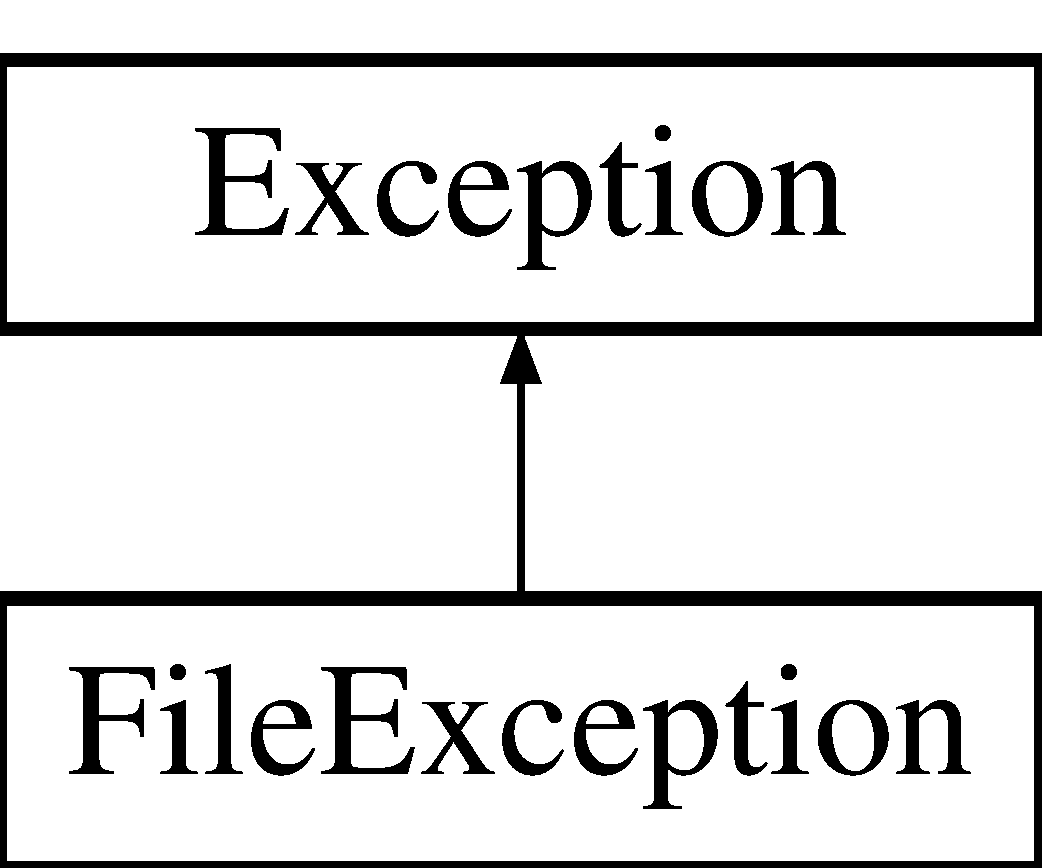
\includegraphics[height=2.000000cm]{classFileException}
\end{center}
\end{figure}


\subsection{Detailed Description}
\hyperlink{classFileException}{FileException} occurs when requesting /file fails. 

Definition at line 36 of file exceptions.php.



The documentation for this class was generated from the following file:\begin{DoxyCompactItemize}
\item 
bayphp/exceptions.php\end{DoxyCompactItemize}

\hypertarget{classRequest}{
\section{Request Class Reference}
\label{classRequest}\index{Request@{Request}}
}


Sends http requests to the Bayfiles API.  


\subsection*{Public Member Functions}
\begin{DoxyCompactItemize}
\item 
\hyperlink{classRequest_a7a3dc4998f1b9c696543c112f34965b5}{\_\-\_\-construct} (\$url, \$user=null)
\begin{DoxyCompactList}\small\item\em \hyperlink{classRequest}{Request} constructor. \end{DoxyCompactList}\item 
\hyperlink{classRequest_a432fdb6b9f7a071ef270d7ec938bf74d}{setMethod} (\$method)
\begin{DoxyCompactList}\small\item\em sets the http request method \end{DoxyCompactList}\item 
\hyperlink{classRequest_a9c5afc9327a6343f2522e580cc156882}{addUploadFile} (\$fieldname, \$filename)
\begin{DoxyCompactList}\small\item\em adds a file to upload when calling \hyperlink{classRequest_a9716d01ed89fa00bfb6accd5dea70690}{send()} method \end{DoxyCompactList}\item 
\hyperlink{classRequest_a9716d01ed89fa00bfb6accd5dea70690}{send} (\$errorType=null)
\begin{DoxyCompactList}\small\item\em sends the request \end{DoxyCompactList}\item 
\hyperlink{classRequest_a73eb2c038803d2a08ef20235684d8db7}{hasError} ()
\begin{DoxyCompactList}\small\item\em returns whether the request failed \end{DoxyCompactList}\item 
\hyperlink{classRequest_a293e3cf982bf561bc173dd4da46bf305}{getError} ()
\begin{DoxyCompactList}\small\item\em returns the error message given by the error field of the json response \end{DoxyCompactList}\item 
\hyperlink{classRequest_a58b89ed8e9d25ff84259cd19077f88d6}{getResponse} (\$key=null)
\begin{DoxyCompactList}\small\item\em the parsed json response \end{DoxyCompactList}\item 
\hyperlink{classRequest_a6bd35712e69a808c3c3b66fc7ec5986b}{getUrl} ()
\begin{DoxyCompactList}\small\item\em the request url \end{DoxyCompactList}\end{DoxyCompactItemize}


\subsection{Detailed Description}
Sends http requests to the Bayfiles API. 

Definition at line 10 of file request.php.



\subsection{Constructor \& Destructor Documentation}
\hypertarget{classRequest_a7a3dc4998f1b9c696543c112f34965b5}{
\index{Request@{Request}!\_\-\_\-construct@{\_\-\_\-construct}}
\index{\_\-\_\-construct@{\_\-\_\-construct}!Request@{Request}}
\subsubsection[{\_\-\_\-construct}]{\setlength{\rightskip}{0pt plus 5cm}Request::\_\-\_\-construct (
\begin{DoxyParamCaption}
\item[{\$}]{url, }
\item[{\$}]{user = {\ttfamily null}}
\end{DoxyParamCaption}
)}}
\label{classRequest_a7a3dc4998f1b9c696543c112f34965b5}


\hyperlink{classRequest}{Request} constructor. 


\begin{DoxyParams}{Parameters}
{\em url} & the request url, without the base url nor the ?session=xxx suffix \\
\hline
{\em user} & if provided, the request is sent using a specific account \\
\hline
\end{DoxyParams}


Definition at line 24 of file request.php.



\subsection{Member Function Documentation}
\hypertarget{classRequest_a9c5afc9327a6343f2522e580cc156882}{
\index{Request@{Request}!addUploadFile@{addUploadFile}}
\index{addUploadFile@{addUploadFile}!Request@{Request}}
\subsubsection[{addUploadFile}]{\setlength{\rightskip}{0pt plus 5cm}Request::addUploadFile (
\begin{DoxyParamCaption}
\item[{\$}]{fieldname, }
\item[{\$}]{filename}
\end{DoxyParamCaption}
)}}
\label{classRequest_a9c5afc9327a6343f2522e580cc156882}


adds a file to upload when calling \hyperlink{classRequest_a9716d01ed89fa00bfb6accd5dea70690}{send()} method 


\begin{DoxyParams}{Parameters}
{\em fieldname} & \\
\hline
{\em filename} & name of the local file \\
\hline
\end{DoxyParams}


Definition at line 55 of file request.php.

\hypertarget{classRequest_a293e3cf982bf561bc173dd4da46bf305}{
\index{Request@{Request}!getError@{getError}}
\index{getError@{getError}!Request@{Request}}
\subsubsection[{getError}]{\setlength{\rightskip}{0pt plus 5cm}Request::getError (
\begin{DoxyParamCaption}
{}
\end{DoxyParamCaption}
)}}
\label{classRequest_a293e3cf982bf561bc173dd4da46bf305}


returns the error message given by the error field of the json response 

\begin{DoxyReturn}{Returns}
a string containing the error message 
\end{DoxyReturn}


Definition at line 104 of file request.php.

\hypertarget{classRequest_a58b89ed8e9d25ff84259cd19077f88d6}{
\index{Request@{Request}!getResponse@{getResponse}}
\index{getResponse@{getResponse}!Request@{Request}}
\subsubsection[{getResponse}]{\setlength{\rightskip}{0pt plus 5cm}Request::getResponse (
\begin{DoxyParamCaption}
\item[{\$}]{key = {\ttfamily null}}
\end{DoxyParamCaption}
)}}
\label{classRequest_a58b89ed8e9d25ff84259cd19077f88d6}


the parsed json response 

\begin{DoxyReturn}{Returns}
an stdClass object read from the json string 
\end{DoxyReturn}


Definition at line 114 of file request.php.

\hypertarget{classRequest_a6bd35712e69a808c3c3b66fc7ec5986b}{
\index{Request@{Request}!getUrl@{getUrl}}
\index{getUrl@{getUrl}!Request@{Request}}
\subsubsection[{getUrl}]{\setlength{\rightskip}{0pt plus 5cm}Request::getUrl (
\begin{DoxyParamCaption}
{}
\end{DoxyParamCaption}
)}}
\label{classRequest_a6bd35712e69a808c3c3b66fc7ec5986b}


the request url 

\begin{DoxyReturn}{Returns}
the request url composed of the base url (\href{http://api.bayfiles.com/v1}{\tt http://api.bayfiles.com/v1}), the request and optionaly a ?session=xxx suffix 
\end{DoxyReturn}


Definition at line 124 of file request.php.

\hypertarget{classRequest_a73eb2c038803d2a08ef20235684d8db7}{
\index{Request@{Request}!hasError@{hasError}}
\index{hasError@{hasError}!Request@{Request}}
\subsubsection[{hasError}]{\setlength{\rightskip}{0pt plus 5cm}Request::hasError (
\begin{DoxyParamCaption}
{}
\end{DoxyParamCaption}
)}}
\label{classRequest_a73eb2c038803d2a08ef20235684d8db7}


returns whether the request failed 

\begin{DoxyReturn}{Returns}
a boolean meaning if the error message was empty or not after the request 
\end{DoxyReturn}


Definition at line 94 of file request.php.

\hypertarget{classRequest_a9716d01ed89fa00bfb6accd5dea70690}{
\index{Request@{Request}!send@{send}}
\index{send@{send}!Request@{Request}}
\subsubsection[{send}]{\setlength{\rightskip}{0pt plus 5cm}Request::send (
\begin{DoxyParamCaption}
\item[{\$}]{errorType = {\ttfamily null}}
\end{DoxyParamCaption}
)}}
\label{classRequest_a9716d01ed89fa00bfb6accd5dea70690}


sends the request 


\begin{DoxyParams}{Parameters}
{\em errorType} & if given, any error throws an exception of the given type, returns the error message instead \\
\hline
\end{DoxyParams}
\begin{DoxyReturn}{Returns}
the error message or an empty string if errorType is null 
\end{DoxyReturn}


Definition at line 66 of file request.php.

\hypertarget{classRequest_a432fdb6b9f7a071ef270d7ec938bf74d}{
\index{Request@{Request}!setMethod@{setMethod}}
\index{setMethod@{setMethod}!Request@{Request}}
\subsubsection[{setMethod}]{\setlength{\rightskip}{0pt plus 5cm}Request::setMethod (
\begin{DoxyParamCaption}
\item[{\$}]{method}
\end{DoxyParamCaption}
)}}
\label{classRequest_a432fdb6b9f7a071ef270d7ec938bf74d}


sets the http request method 


\begin{DoxyParams}{Parameters}
{\em method} & http method, should be HTTP\_\-METH\_\-GET or HTTP\_\-METH\_\-POST \\
\hline
\end{DoxyParams}


Definition at line 44 of file request.php.



The documentation for this class was generated from the following file:\begin{DoxyCompactItemize}
\item 
bayphp/request.php\end{DoxyCompactItemize}

\hypertarget{classUploader}{
\section{Uploader Class Reference}
\label{classUploader}\index{Uploader@{Uploader}}
}


Class for uploading files.  


\subsection*{Public Member Functions}
\begin{DoxyCompactItemize}
\item 
\hypertarget{classUploader_a60c2d30006a87612fb93977b58d5ba89}{
\hyperlink{classUploader_a60c2d30006a87612fb93977b58d5ba89}{\_\-\_\-construct} ()}
\label{classUploader_a60c2d30006a87612fb93977b58d5ba89}

\begin{DoxyCompactList}\small\item\em \hyperlink{classUploader}{Uploader} constructor. \end{DoxyCompactList}\item 
\hypertarget{classUploader_ad89a94d5f36bdeadd4e97d1114f2dd3b}{
\hyperlink{classUploader_ad89a94d5f36bdeadd4e97d1114f2dd3b}{prepare} (\$owner=null)}
\label{classUploader_ad89a94d5f36bdeadd4e97d1114f2dd3b}

\begin{DoxyCompactList}\small\item\em call it before \hyperlink{classUploader_af16f57142f7a015461a51f26cd786f5d}{send()} in order to get the upload and progress urls \end{DoxyCompactList}\item 
\hypertarget{classUploader_aa1d13a8f40e54cb73fa3d5cd12d4794d}{
\hyperlink{classUploader_aa1d13a8f40e54cb73fa3d5cd12d4794d}{getUploadUrl} ()}
\label{classUploader_aa1d13a8f40e54cb73fa3d5cd12d4794d}

\begin{DoxyCompactList}\small\item\em upload url getter \end{DoxyCompactList}\item 
\hypertarget{classUploader_ab908cff6cbdf2b5af26da7815e3f3a13}{
\hyperlink{classUploader_ab908cff6cbdf2b5af26da7815e3f3a13}{getProgressUrl} ()}
\label{classUploader_ab908cff6cbdf2b5af26da7815e3f3a13}

\begin{DoxyCompactList}\small\item\em progress url getter \end{DoxyCompactList}\item 
\hypertarget{classUploader_af16f57142f7a015461a51f26cd786f5d}{
\hyperlink{classUploader_af16f57142f7a015461a51f26cd786f5d}{send} (\$filename, \$owner=null)}
\label{classUploader_af16f57142f7a015461a51f26cd786f5d}

\begin{DoxyCompactList}\small\item\em sends the file and returns it as a \hyperlink{classFile}{File} instance \end{DoxyCompactList}\end{DoxyCompactItemize}


\subsection{Detailed Description}
Class for uploading files. 

Definition at line 10 of file uploader.php.



The documentation for this class was generated from the following file:\begin{DoxyCompactItemize}
\item 
bayphp/uploader.php\end{DoxyCompactItemize}

\printindex
\end{document}
